\documentclass[11pt]{article}
\usepackage[margin=1in]{geometry}

% Packages we need
\usepackage{amsmath}
\usepackage{amsfonts}
\usepackage{mathtools}
\usepackage{amsthm}
\usepackage{float}
\usepackage{graphicx}
\usepackage{listings}
\usepackage{color} %red, green, blue, yellow, cyan, magenta, black, white

% Header packages
\usepackage{fancyhdr}
\fancyhf{}
\pagestyle{fancy}


% Formatting document
\setcounter{secnumdepth}{0}
\setlength{\parindent}{0in}
\setlength{\parskip}{0.5em}

% MATLAB code
\definecolor{mygreen}{RGB}{28,172,0} % color values Red, Green, Blue
\definecolor{mylilas}{RGB}{170,55,241}

% Commands
\DeclarePairedDelimiter\ceil{\lceil}{\rceil}
\DeclarePairedDelimiter\floor{\lfloor}{\rfloor}
\newcommand{\ws}{\text{ }}
\newcommand{\e}[1]{\times 10^{#1}}

% Header
\lhead{\textsc{CS 5220 -- Project 1}} % TODO: enter title here
\rhead{\textsc{Eric Gao -- emg222\\Junteng Jia -- jj585}} % Authors
\setlength{\headheight}{0.5in}
\cfoot{\thepage}

% Title
\title{CS 5220 -- Project 1} %TODO: enter title here
\author{
  \begin{tabular}{l c l}
    Eric Gao & -- & emg222\\
    Junteng Jia & -- & jj585
  \end{tabular}\\
  \rule{\linewidth}{0.4pt}
}
\date{}

\lstset
{
    frame=tb,
    language=C++,
    aboveskip=3mm,
    belowskip=3mm,
    showstringspaces=false,
    columns=flexible,
    basicstyle={\small\ttfamily},
    numbers=none,
    numberstyle=\tiny\color{gray},
    keywordstyle=\color{blue},
    commentstyle=\color{dkgreen},
    stringstyle=\color{mauve},
    breaklines=true,
    breakatwhitespace=true,
    tabsize=4
}




\begin{document}
    \thispagestyle{empty}
    \maketitle

    \vspace{1cm}

    \begin{figure}[H]
        \centering
        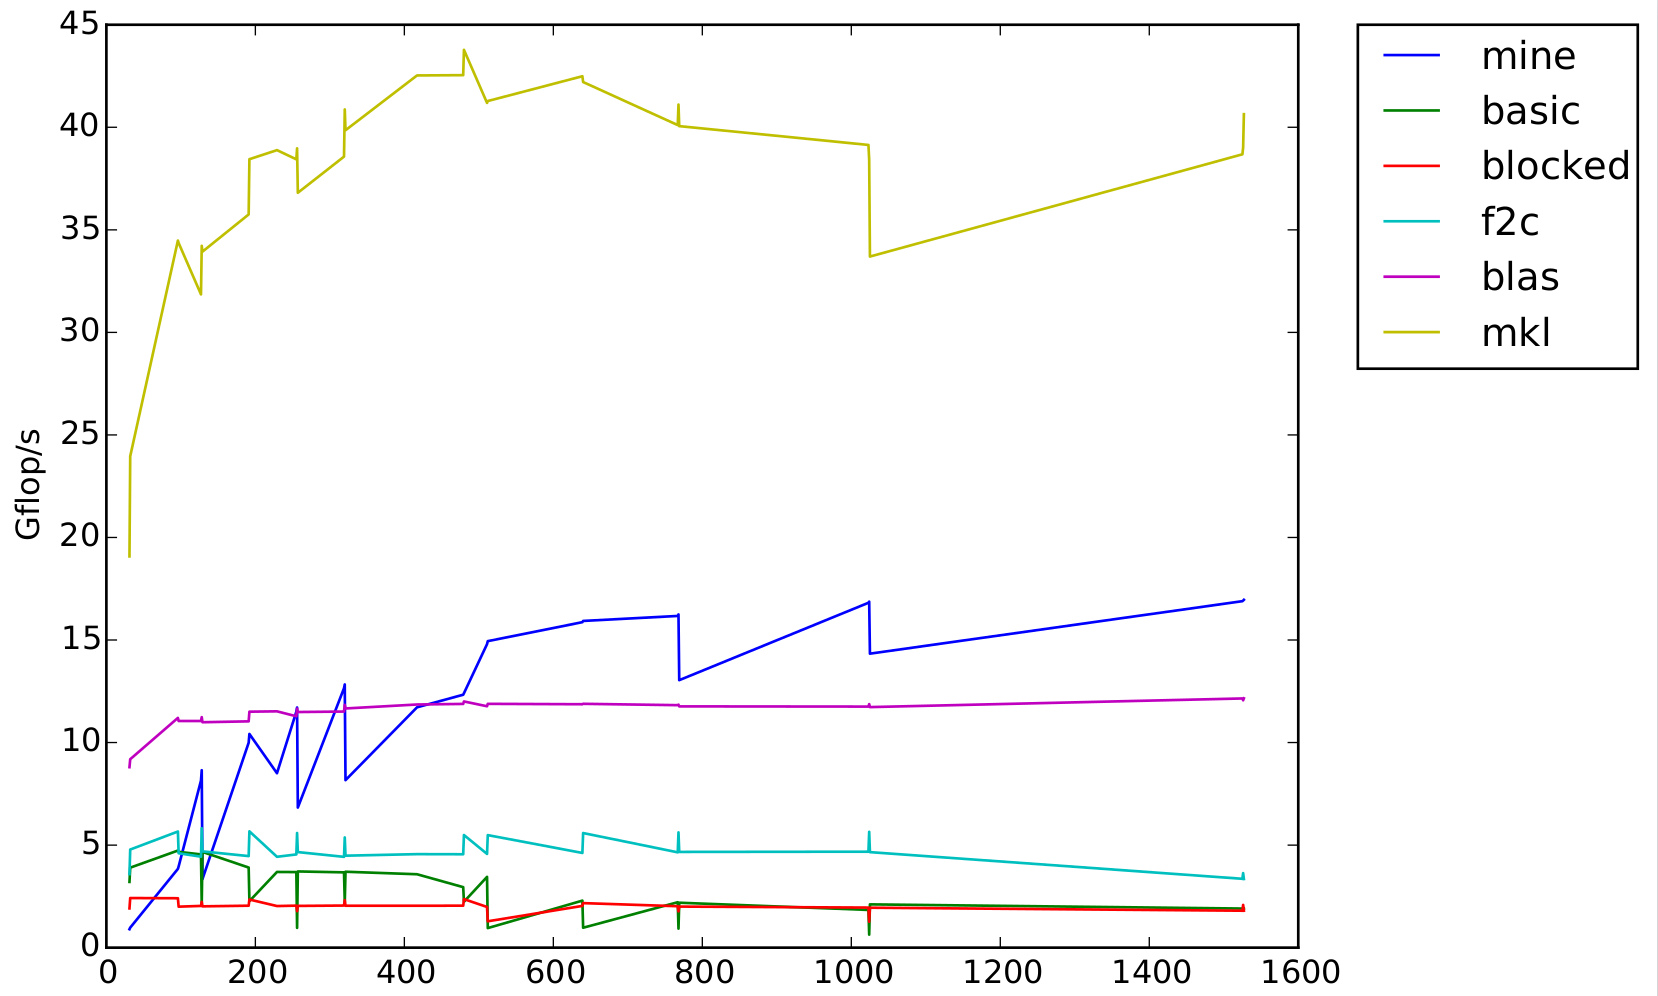
\includegraphics[width=6.5in]{timing_vector_32_64_cc_cp_align.png}
        
        \begin{center}
        We wrote this code from scratch and we beat blas :)         
        \end{center}
    \end{figure}


    \clearpage

    \tableofcontents\

    \pagebreak
    \section{Our approach}
    We made six major improvements:
     \begin{enumerate}
            \item Block multiplication.
            \item Copy optimization.
            \item Vectorization.
            \item Data alignment.
            \item Further blocking
            \item Compiler optimization
     \end{enumerate}
    
        \vspace{1cm}
                
        \subsection{Block multiplication}
        We split the matrices into several blocks. We chose the blocks to be size 32, which means that each block takes up 8KB ($32^2 * 8$). This means we can fit all three blocks of the three matrices we care about into the L1 cache of the Phi processors since the L1 cache is 32KB. As a result, we can write a very fast kernel that allows us to take advantage of the fact that we know the size of the matrix and the fact that everything is in the L1 cache. This way, we can unroll our loops so we don't have to make unnecessary branching operations. We can then use this fast kernel to multiply blocks together so that we get the final result.
        
        \begin{figure}[H]
            \centering
            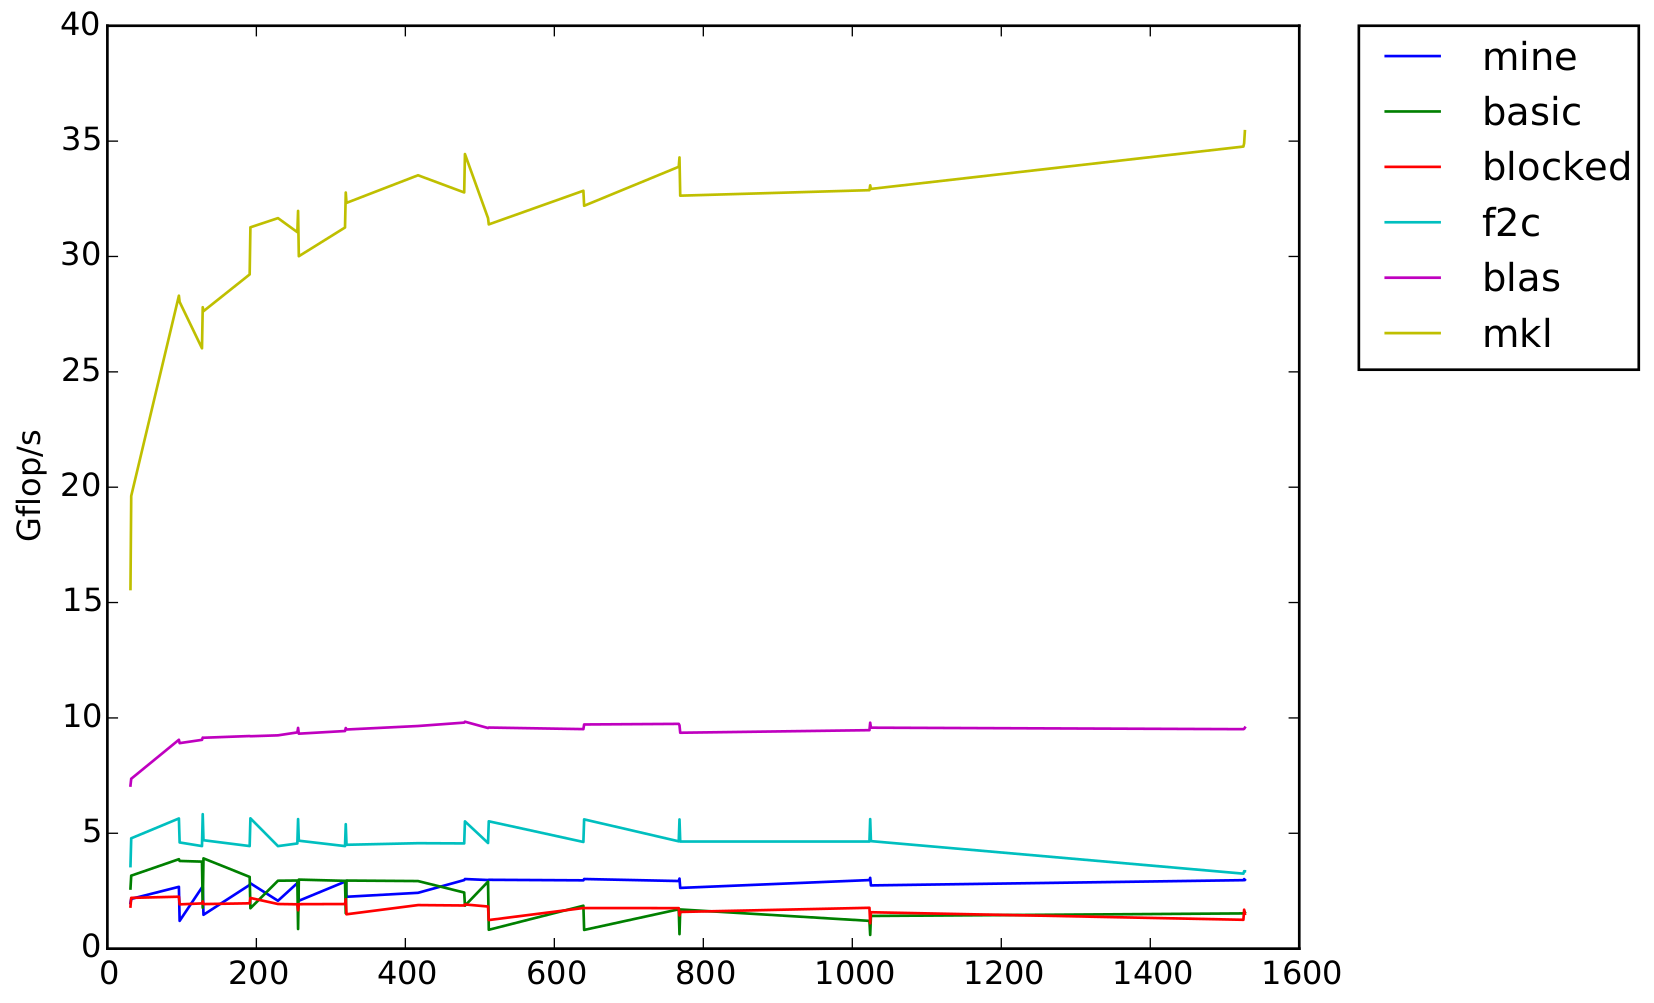
\includegraphics[width=4.5in]{timing_32.png}
            \caption{After block multiplication}
        \end{figure}
        
        \clearpage
        
    
        
        \subsection{Copy Optimization}
        We arranged the data so that within each block of $A$, the entries are row major and the blocks themselves are arranged in row major order. For $B$, the entries in the block are row major and the blocks themselve are arranged in column major order. We arrange them in this order so that we can have a stride of 1 for our kernel. This is to maximize spatial locality.
        
        Also, by doing this, we can handle fringe cases well. We make sure that matrices that we are multiplying have a leading dimension that is a multiple of our block size. We just add zeros on the edges to ensure this.
        
        \begin{figure}[H]
            \centering
            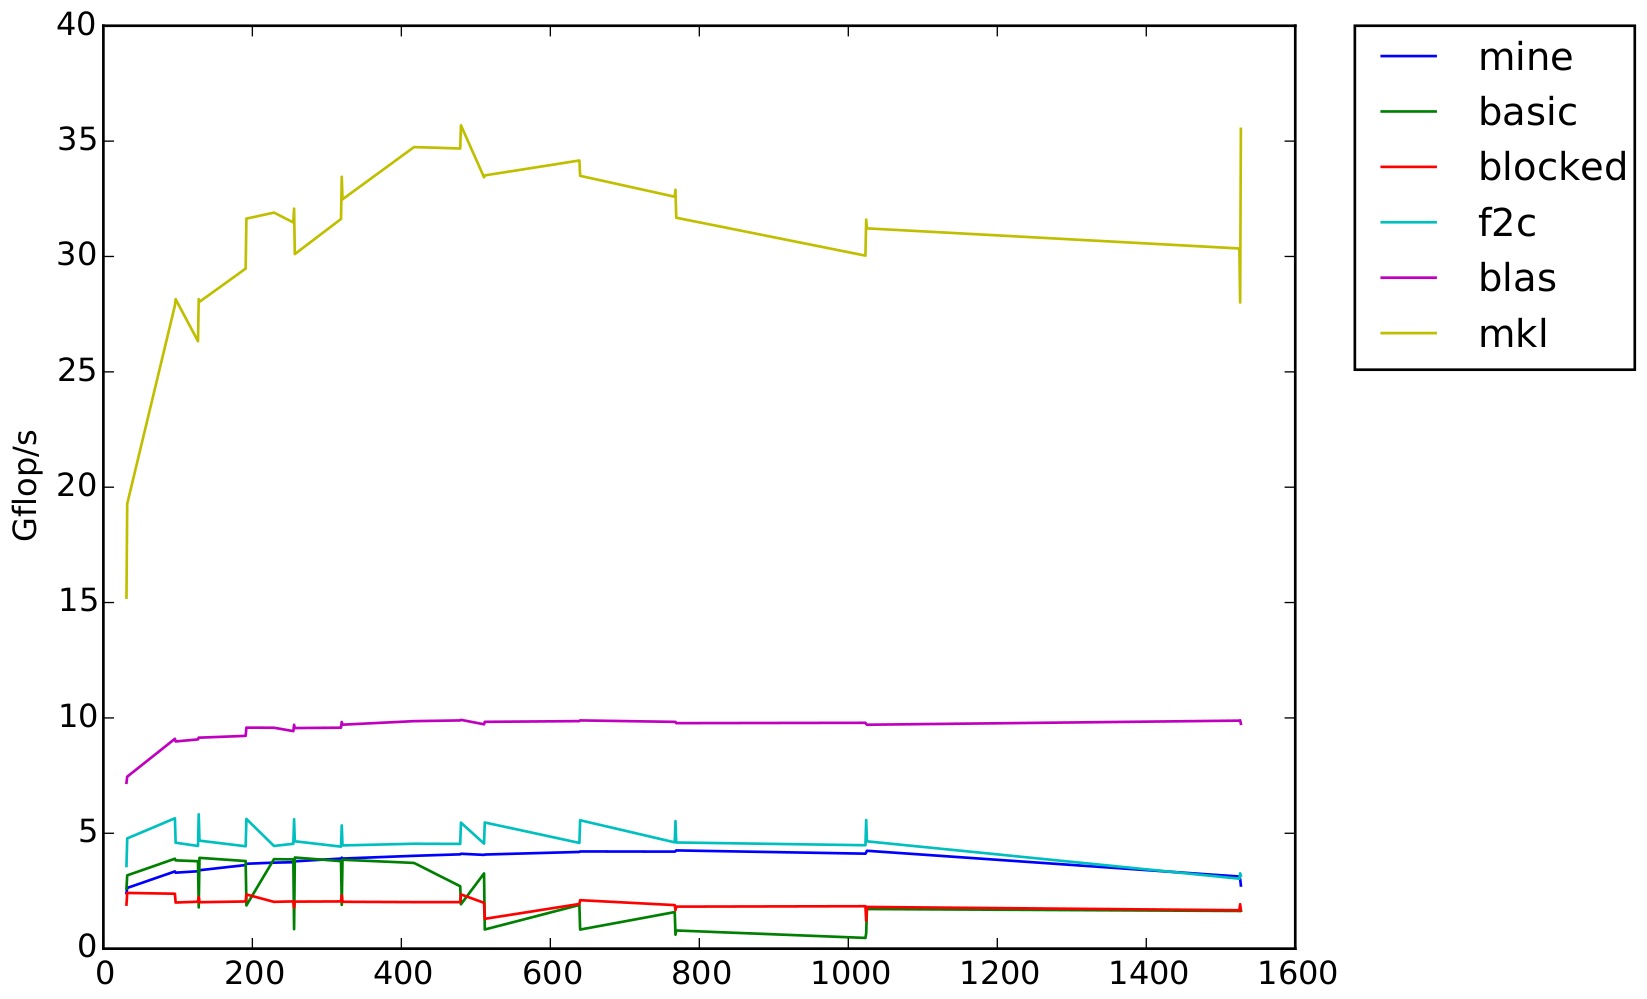
\includegraphics[width=4.5in]{timing_32_cp.png}
            \caption{After copy optimization}
        \end{figure}
        
        \clearpage
            
    
                
        \subsection{Vectorization}
        We aligned our data to 64 bytes in memory and we multiply the blocks in our matrices in such an order so that we can take advantage of Vector FMAs. Specifically, we start with the (0, 0) element of a block in $A$. We multiply that by the first row of a block in $B$. We add that to the first row of a block in $C$. We then iterate across the 0th row of $A$ and iterate over the rows of the block in $B$. Then our outer loop iterates over the rows of $A$. This way, on our inner loop, we can take advantage of vector operations. When we compiled our code with the flags to show us whether we have vectorization, we obtained the following output:
        
        \vspace{1cm}
        
        \begin{lstlisting}
        LOOP BEGIN at dgemm_mine.c(121,13) inlined into dgemm_mine.c(199,17)
        remark #15388: vectorization support: reference C_row.286 has aligned access
        remark #15388: vectorization support: reference C_row.286 has aligned access
        remark #15388: vectorization support: reference B_row.288 has aligned access
        remark #15399: vectorization support: unroll factor set to 8
        remark #15300: LOOP WAS VECTORIZED
        remark #15448: unmasked aligned unit stride loads: 2 
        remark #15449: unmasked aligned unit stride stores: 1 
        remark #15475: --- begin vector loop cost summary ---
        remark #15476: scalar loop cost: 13 
        remark #15477: vector loop cost: 4.000 
        remark #15478: estimated potential speedup: 3.220 
        remark #15479: lightweight vector operations: 6 
        remark #15480: medium-overhead vector operations: 1 
        remark #15488: --- end vector loop cost summary ---
        LOOP END
        \end{lstlisting}
        
        \vspace{0.5cm}

        \begin{figure}[H]
            \centering
            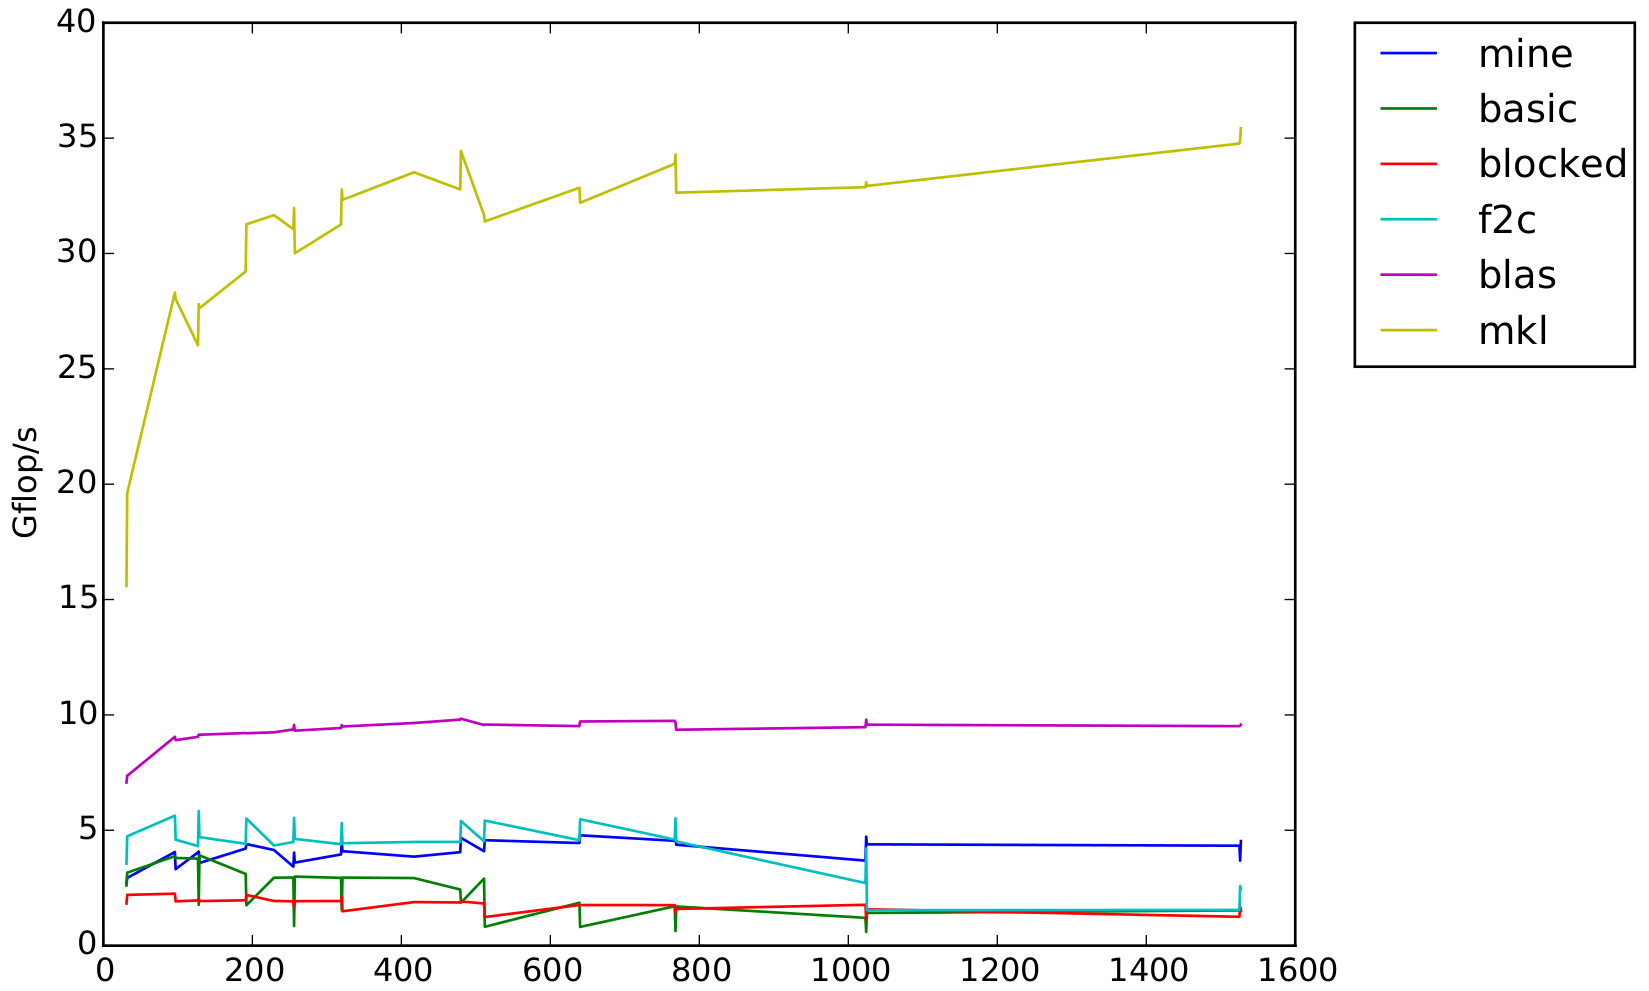
\includegraphics[width=4.5in]{timing_vector_32_cp.png}
            \caption{After vectoriztion}
        \end{figure}
        
        \clearpage
        
    
                    
        \subsection{Data alignment}
        We used the functions \texttt{\_mm\_malloc()} and \texttt{\_mm\_free()} so that we can guarantee that our matrices are aligned properly in memory. Specifically, we ensure that they are aligned to 64 bytes. We do this to ensure that we can take advantage of vector operations.
        
        \begin{figure}[H]
            \centering
            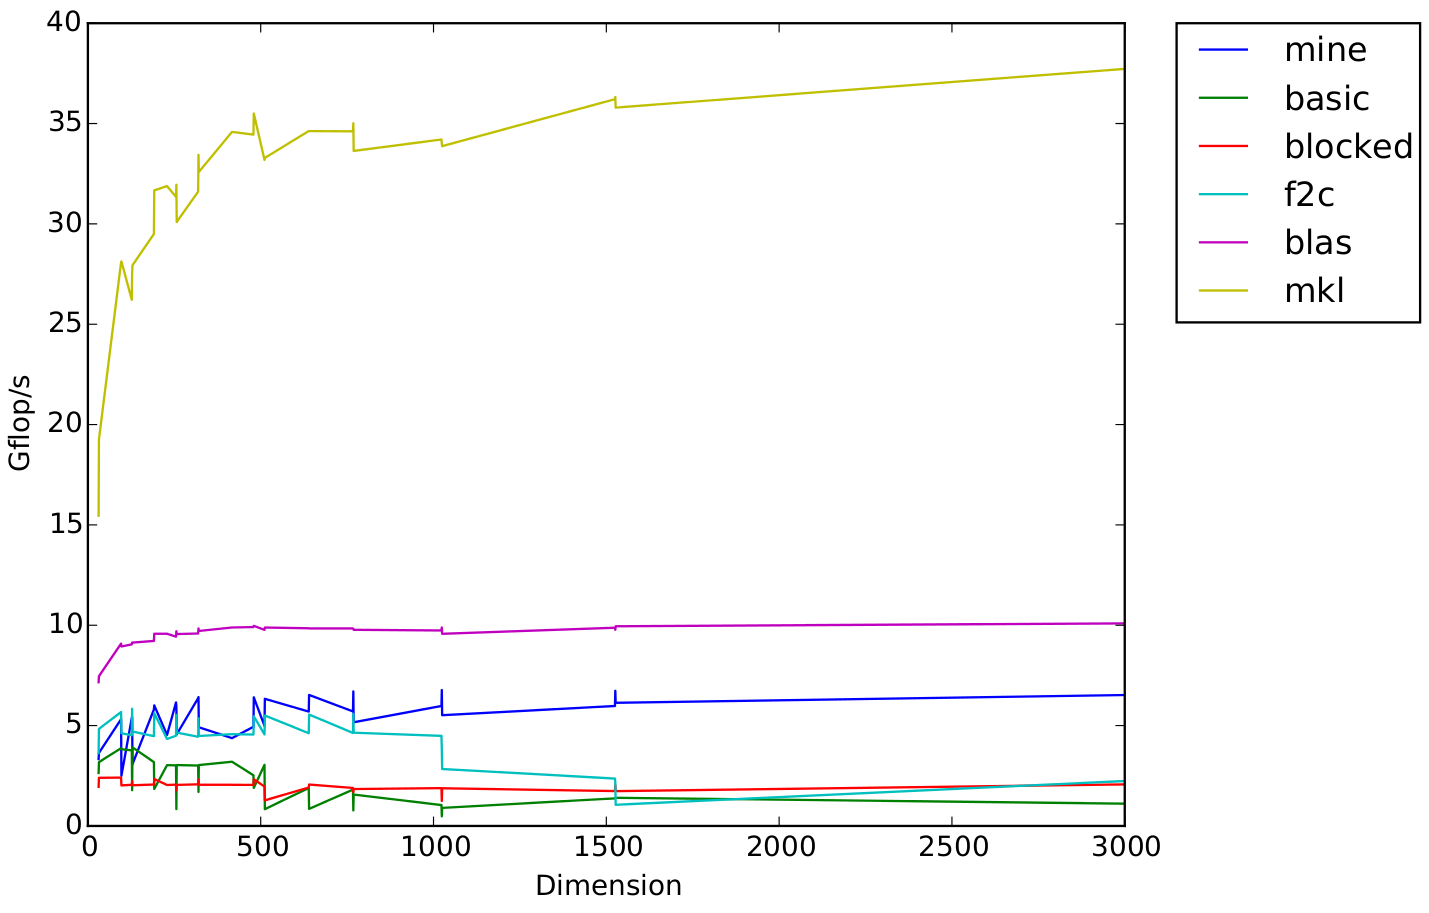
\includegraphics[width=4.5in]{timing_vector_32_cp_align.png}
            \caption{After data alignment}
        \end{figure}
        
        
        
        \subsection{Further blocking}
        
        \begin{figure}[H]
            \centering
            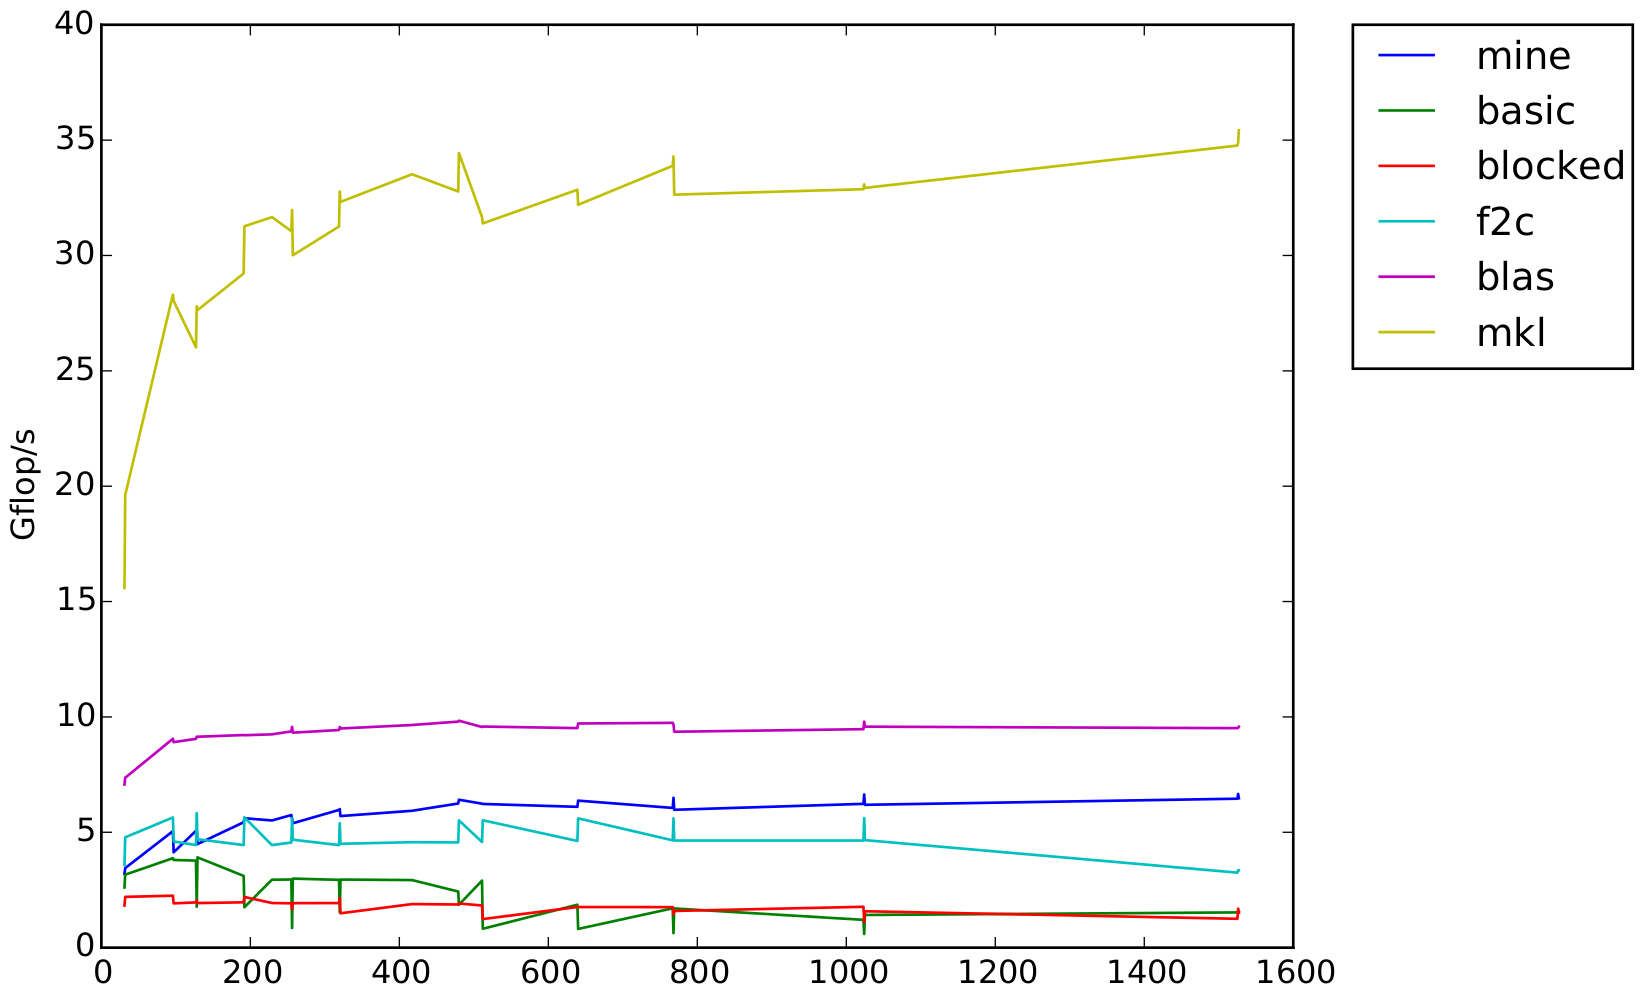
\includegraphics[width=5in]{timing_vector_32_64_cp_align.png}
            \caption{After further blocking}
        \end{figure}
        
        \clearpage
                        
        
            
        \subsection{Compiler optimization}
        
        \vspace{0.5cm}
        
        To fully utilize the power of intel compiler, we used the following compiler flag:
        \begin{center}
        \texttt{-O3 -fast -axCORE-AVX2 -unroll-aggressive -mtune=core-avx2 -ipo -xHost} 
        \end{center}
        
        \begin{itemize}
            \item The 03 flag tells the optimizer to perform aggressive optimizations.
            \item The unroll-aggressive is a intel compiler option that tells the compiler to unroll the loops that the compiler believes would lead to a speed up. 
            \item The ipo flags tells the compiler to do interprocedure optimizations, so this means that the compiler is going to attempt to reduce the amount of time that exists when functions are in different files.
            \item The xHost flag applies a high level vectorization to the code.
            \item The axCORE-AVX2  and mtune$=$core-avx2 flags tell the compiler to take advantage of the fact that our CPU has access to the AVX2 vectorization operations, and therefore we want our code to be tuned to this AVX2 instruction set. 
        \end{itemize}
        
        Using compiler optimization is what we learned from group 20 and group 24 during peer review.
        
        \vspace{1cm}
        
        \begin{figure}[H]
                \centering
                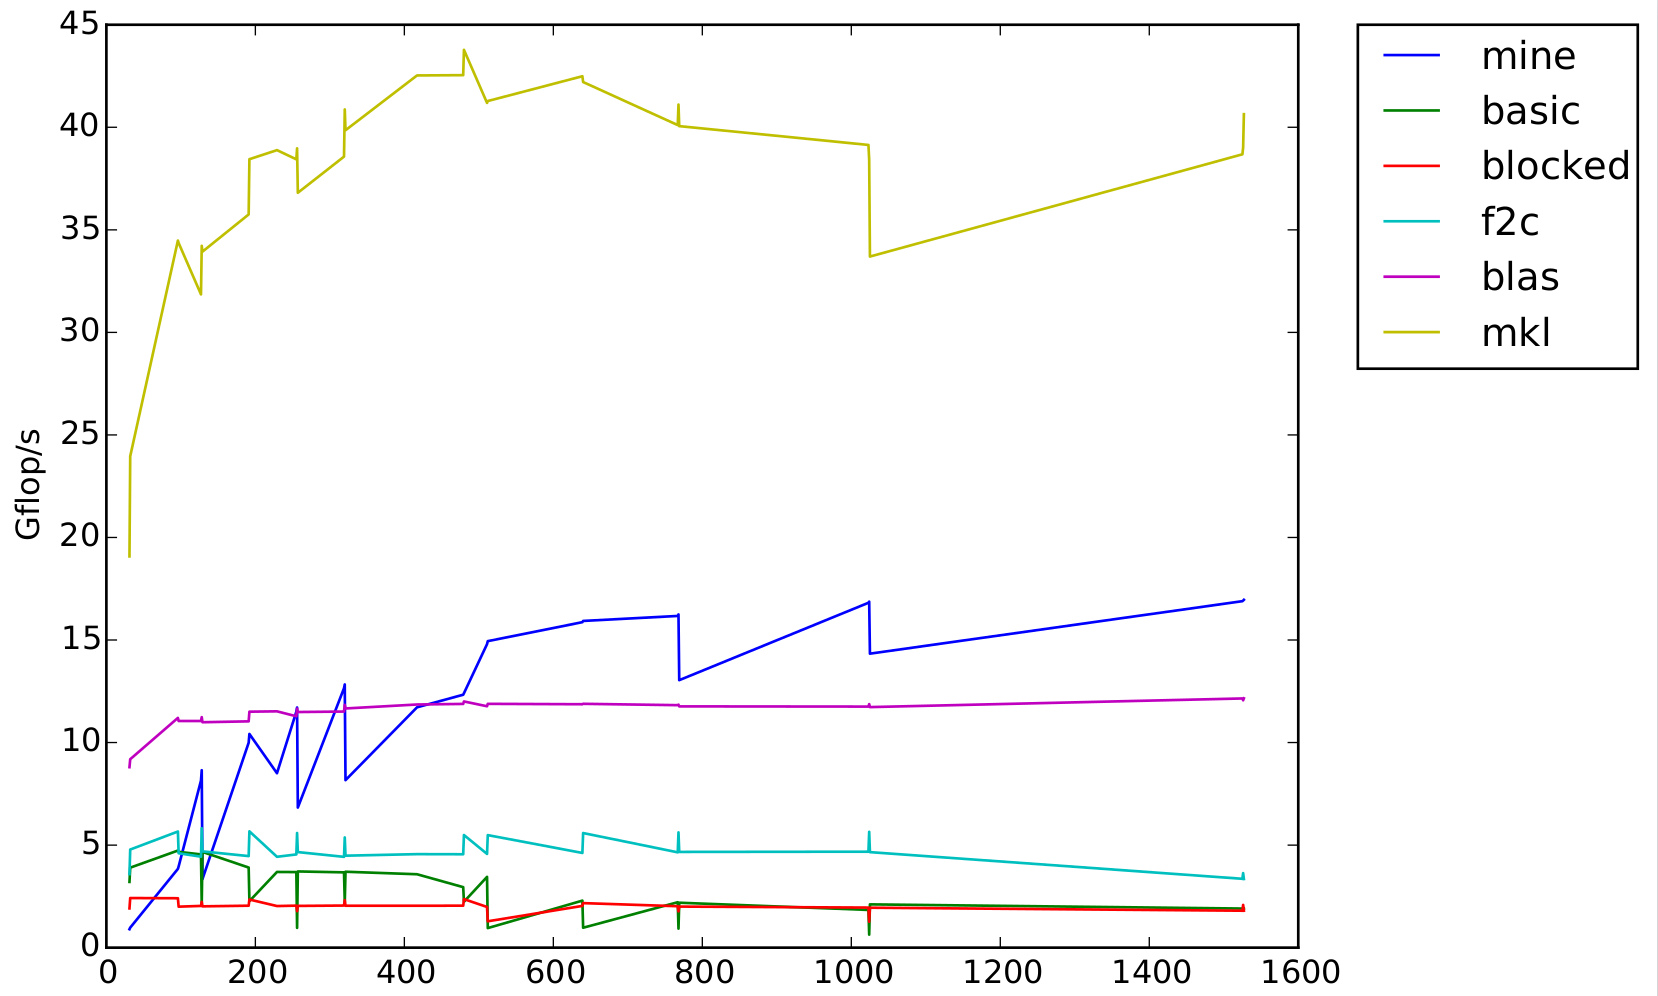
\includegraphics[width=4.5in]{timing_vector_32_64_cc_cp_align.png}
                \caption{After compiler optimization}
        \end{figure}
        
        \clearpage  
        

        \subsection{L2 blocking}

        We then implemented a multi-level blocking strategy. We first divided the matrices into blocks so that each block could fit into the L1 cache. We then created larger blocks that contained several smaller blocks and performed a block matrix multiply using those larger blocks. We created the larger blocks that contained larger submatrices that could fit into the L2 cache.  Specifically, we had 4 smaller blocks in every larger block, resulting in a matrix of 64 x 64 doubles if our smaller blocks were 32 x 32 doubles. The result of this had a minor improvement on performance for larger matrices. The overhead of the copy optimization resulted in lower FLOP rates for smaller matrices. The results are seen below:
        \begin{figure}[H]
            \centering
            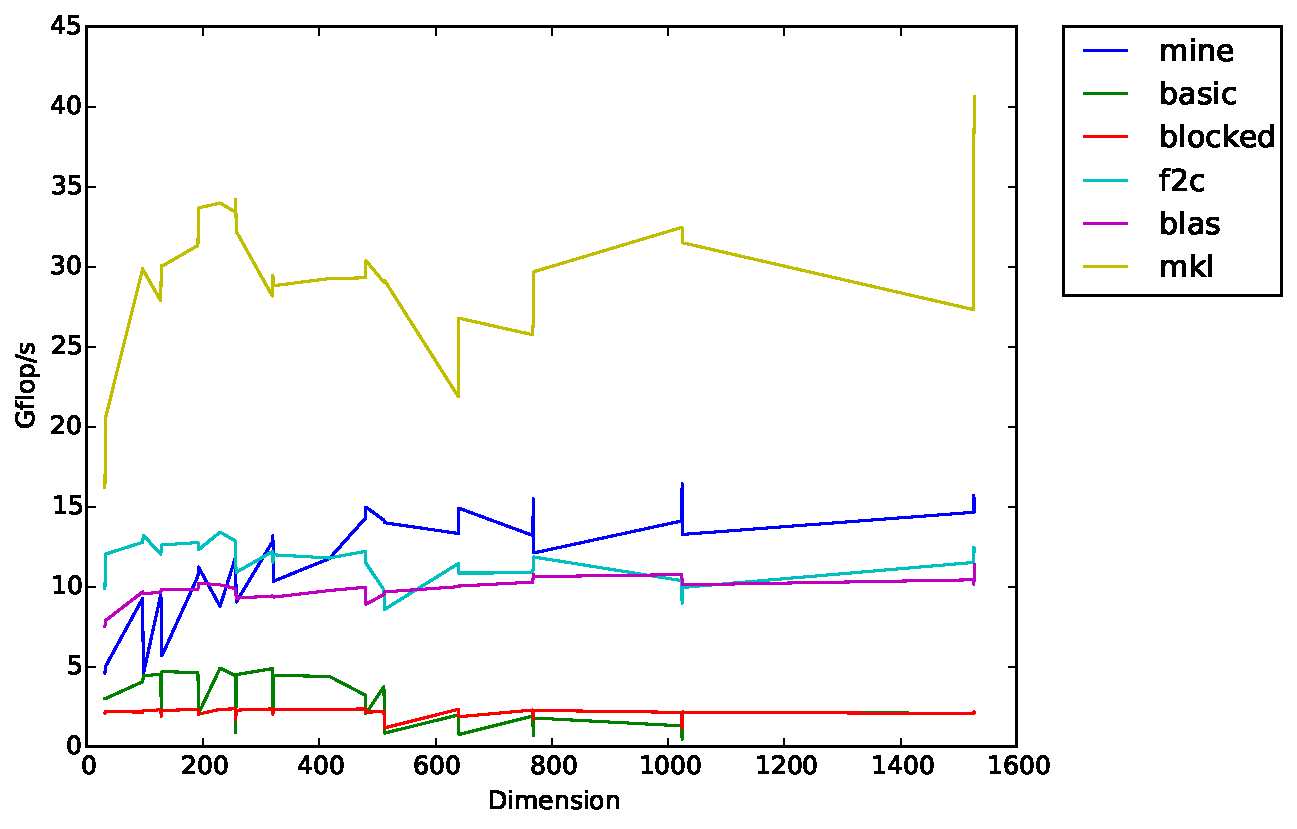
\includegraphics[width=4.5in]{timing_noL2.pdf}
            \caption{Without L2 blocking.}
        \end{figure}

        \begin{figure}[H]
            \centering
            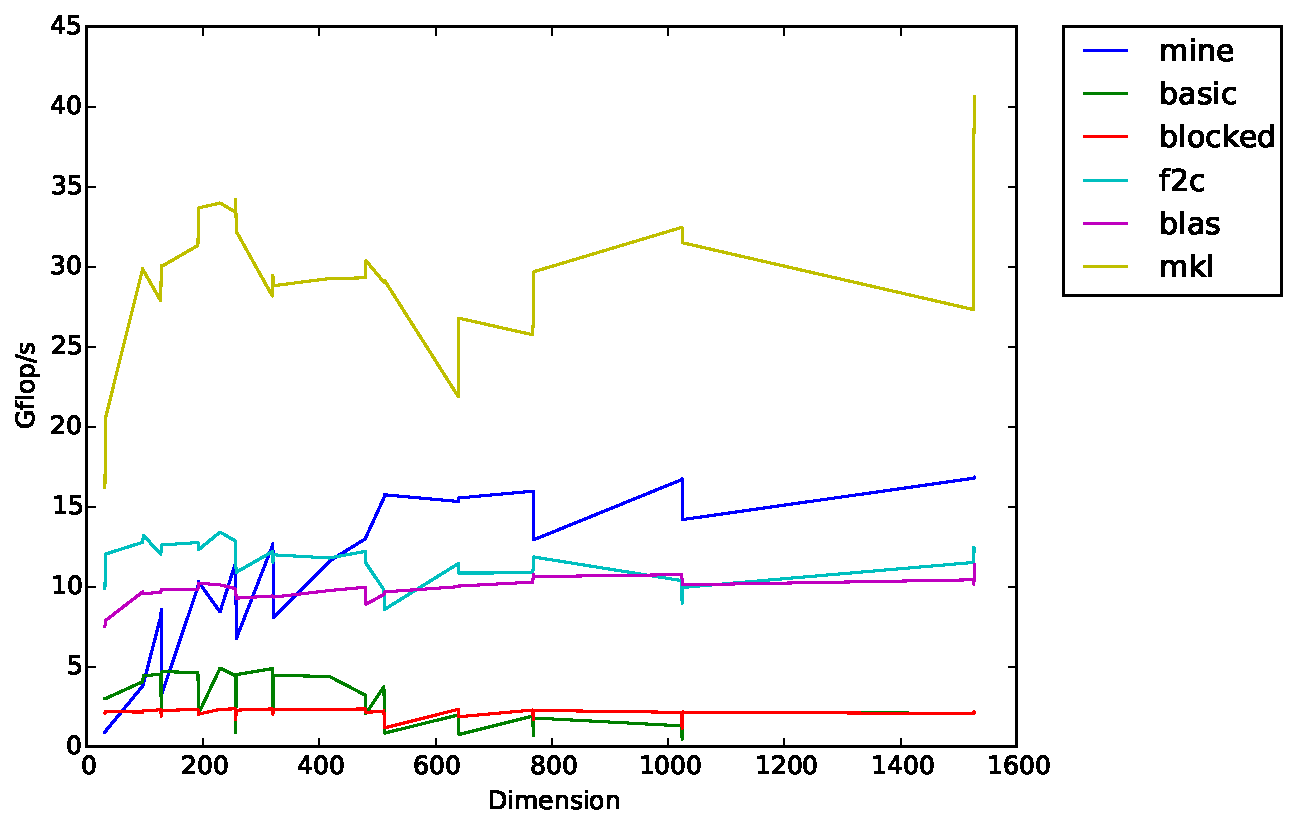
\includegraphics[width=4.5in]{timing_L2.pdf}
            \caption{With L2 blocking. Notice that the FLOP rate is marginally higher for larger matrices but lower for smaller matrices.}
        \end{figure}

        Looking at this, we can try just branching based on the size of the input matrix, which isn't too expensive since it is being done outside of all loops. When we do this, we get the following result. However, the compiler cannot optimize a lot of the code out if we are doing this conditional branching. This causes the overall result to be worse.
        \begin{figure}[H]
            \centering
            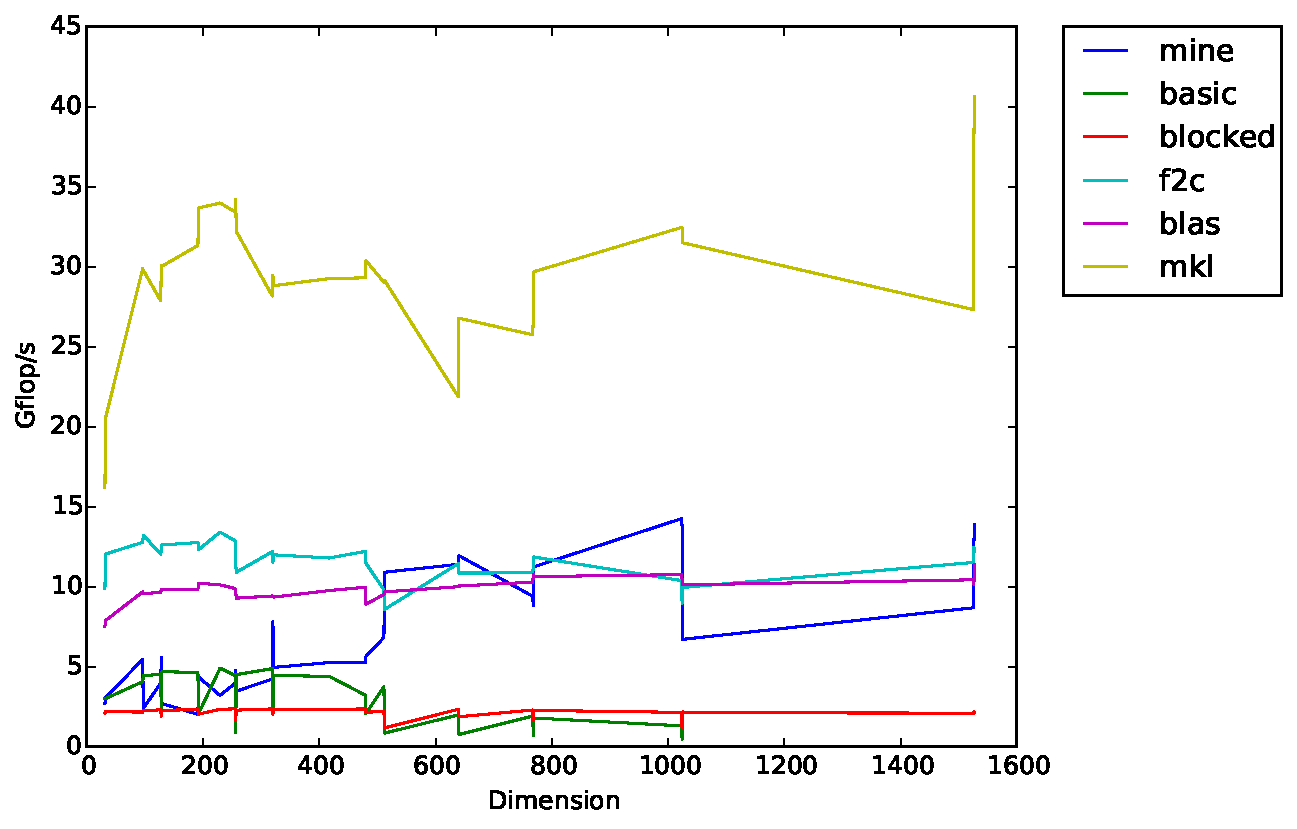
\includegraphics[width=4.5in]{timing_L2_2.pdf}
            \caption{With L2 blocking but branching to use L2 blocking only if the size of the leading dimension of the matrix is greater than 384.}
        \end{figure}

        \clearpage
    \section{Summary}
        
    Through this project, we learned:
    \begin{itemize}
        \item Library functions such as mkl is very well optimized, we should use those libraries as building blocks when we are coding.
        \item Whether we can fully utilize vector ALU will decide the performance of our serial code.
        \item Thinking about the data transfer in cache and register while we are coding can gain us a lot performance.
        \item Intel compiler is amazingly good at optimization, we should take advantage of that.
        \item Peer assessment is interesting and useful. Its a combination of completing and collaborating.
    \end{itemize}

    Our results compared to other matrix multiplication implementation. Our code is comparable to the blas implementation (with out optimization) for smaller matrices and runs faster for larger matrices.

\end{document}